\subsection{Gerarchia degli attori}
\begin{figure}[h]
  \centering
  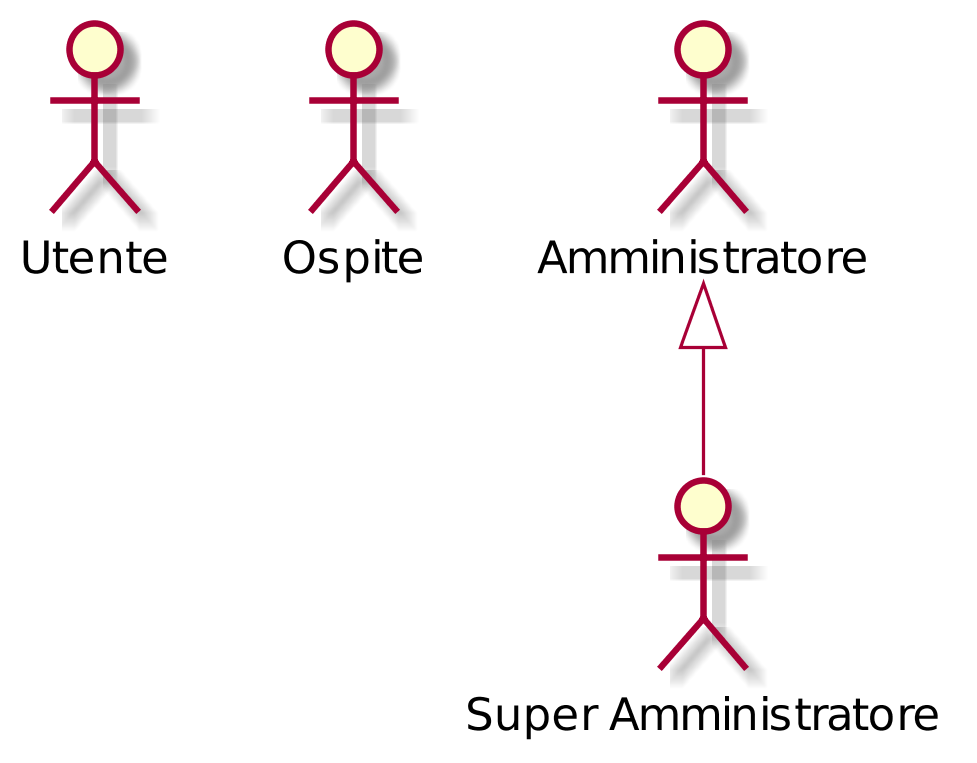
\includegraphics[scale=0.4]{images/Attori.png}
  \caption{Gerarchia degli attori}
\end{figure}
Dopo un'attenta analisi da parte del gruppo gli attori che sono stati individuati sono: 
\begin{itemize}
\item \textbf{Utente}: un utente del \gl{sistema}, il quale non è ancora stato identificato né come amministratore né come ospite;
\item \textbf{Ospite}: ospite esterno, il quale vuole incontrare un membro dell'azienda;
\item \textbf{Amministratore}: membro dell'azienda che dispone dei privilegi di amministrazione, i quali gli permettono di modificare il comportamento del sistema;
\item \textbf{Super Amministratore}: generalizzazione di amministratore, può creare e modificare altri amministratori e dispone di privilegi globali;
\end{itemize}